
\chapter{Mechanical Design}


\section{Overview}
The design of LARRE was inspired by the modular design presented by Bartenbach \textit{et. al.} \cite{7523699}.  Aliman \textit{et. al} also comprised a survey of all the existing lower limb exoskeletons currently in development; the survey gave further insight into the choice of actuators and sensors \cite{aliman2017design}. The Bartenbach design outlined the basic structure for the rehabilitation exoskeleton and improved by integrating additional sensors from the Aliman survey into the system. Additionally, the ankle-foot orthosis was moved to an overshoe joint to allow the system to don and doff with greater ease.
LARRE was designed to be a modular testing platform. Here we define modular as the ability to adjust to a person and allow for the swapping out of the joint mechanisms. LARRE's design fits the following requirements. 


\begin{enumerate}[noitemsep]
\item \textbf{Data Driven}: The kinematics and dynamics of the joints are defined by the biomechanical data. The joints must have the power to compensate for the mass of the person and the exoskeleton. 
\item \textbf{Adjustable}: The exoskeleton must be adjustable to fit the different people in order for the exoskeleton's joints to align properly to avoid putting unnatural force on a person's joints. 
\item \textbf{Modular}: The exoskeleton requires removable joints to allow for different joints testing and experimentation; therefore, universal connectors are needed to allow the swapping out of the joints. 
\item \textbf{Easy to build}: The exoskeleton needs to be easy to manufacture and assemble. The exoskeleton should be constructed from off-the-shelf material to allow researchers to build their testing and development systems. 
\item \textbf{Easy of Use}: The exoskeleton needs to be easy to use for both the clinician and the person wearing the exoskeleton. 
\end{enumerate}

 \autoref{fig:Render} shows an annotated rendering of LARRE.  Each of the major components is discussed in detail in  \autoref{sec:hip}, \autoref{sec:knee}, and \autoref{sec:ankle}. While LARRE was designed to work as a single system, the modality allowed each joint treated as a separate component and be independently designed and tested. 

\begin{figure}[h!]
    \centering
    \includegraphics[scale=0.25]{images/mech_design/rendering2.png}
    \caption{Rendering of exoskeleton.}
    \label{fig:Render}
\end{figure}


\section{Hip Orthosis}
\label{sec:hip}

\autoref{fig:hip} shows an exploded rendering of the LARRE hip. The hip has an extension plate to expand the hips' width; they slide apart and lock with bolts. The bars along the person's back hold the battery box and support the person's upper body. A tactical vest \footnote{https://www.harmonicdrive.net/products/rotary-actuators#5071} and belt \footnote{https://tacticalgear.com/condor-gen-ii-battle-belt-od-green?hp=y}  straps the person into the exoskeleton. This vest and belt were chosen due to their high strength and padding, supporting the exoskeleton's weight and avoiding bruising the person. The belt is connected to LARRE and provides trunk support to help align the hip joints. The hips joints slide back and forth to align LARREs joints with the joints of the person.


\begin{figure}[h!]
    \centering
    \includegraphics[scale=0.15]{images/mech_design/hip.png}
    \caption{Exploded Hip Mechanism}
    \label{fig:hip}
\end{figure}

LARRE is designed to be either passive or active. The passive mode allows the LARRE to be worn and collect data without controlling the motors. The passive version of the exoskeleton has been built for proof of concept. 

The active mode of the LARRE uses Maxon EC90 flat motors \footnote{https://www.maxongroup.com/maxon/view/product/motor/ecmotor/ecflat/ecflat90/505592} connected to Harmonic gearboxes \footnote{https://www.harmonicdrive.net/products/rotary-actuators#5071}. The Maxon motors are compact and have a low profile and built-in encoders. This motor is ideal for use in exoskeletons since it is a hollowed shaft gearbox that does not increase the exoskeletons' width. The encoders allow for positional control of the motors. Harmonic gearboxes reduce backlash and provide a 100:1 gear ratio. The active mode has been designed but left for future work to implement. 

This platform's modality makes it ideal for testing different orthoses because of its' ability to easily switch the joints to test either a passive or active exoskeleton. The hip also acts as the base for the other joint that will be discussed below. 



\section{Wrap Spring Knee Orthosis}
\label{sec:knee}

The work done in this section was in collaboration with  Vishnu Aishwaryan \cite{mani2020design}. I managed the overall mechanical design and the manufacturing process. I also aided in the design and running of the experimental validation.

Despite the body of literature about knee orthosis, only a few report the essential quantitative measurements, such as static or dynamic torque, safety, weight, and size. The lack of critical information made it difficult to arrive at design criteria. The design of the knee orthosis was based on the design criteria, and the trade study found here \cite{subra2020design}. In the trade study, each criterion was assigned a different weight of importance, totaling 100 points, and allowed for the mechanism and parameters for the knee orthosis to be selected. The study concluded that a wrap spring clutch mechanism was the best design due to its highest score. The results are summarized in \autoref{tab:trade}.


\begin{table}[h!]
  \begin{center}
    \begin{tabular}{c|c|c|c} % <-- Alignments: 1st column left, 2nd middle and 3rd right, with vertical lines in between
      \textbf{wrap spring} & \textbf{motor} & \textbf{gears/clutch} & \textbf{cables} \\
      \hline \hline
      832.5 & 627.5 & 752.5 & 675.0 \\
      \hline
      \textbf{SEA}  & \textbf{Wafer disks}  & \textbf{Mag Damper} & \textbf{Hydraulics} \\
      \hline \hline
      592.5 & 805.0 & 757.5 & 580.0\\
    \end{tabular}
  \end{center}
      \caption[Knee Trade Study]{Summery of trade study}
    \label{tab:trade}
\end{table}


A wrap spring clutch mechanism is a quasi passive mechanism that allows for high holding torques \cite{irby1999optimization} \cite{tung2013design}. It consists of an arbor that is concentric with a wrap spring. \autoref{fig:WrapSpringClutch} illustrates how a wrap spring clutch mechanism works. The arbor is designed to have a slightly larger diameter than the spring. The friction between the arbor and spring prevents the arbor from rotating. When the leg's spring is actuated, the spring's diameter increases, allowing the spring to rotate freely. 

\begin{figure}
    \centering
    \includegraphics[scale=0.45]{images/mech_design/wrapspringclutch.png}
    \caption[Wrap Spring Clutch]{Wrap Spring Clutch \cite{irby1999optimization}}
    \label{fig:WrapSpringClutch}
\end{figure}


The knee joint for LARRE uses a wrap spring clutch/brake mechanism. \autoref{fig:kneemechASM} shows the knee casing and components.  \autoref{fig:subknee} shows the primary knee mechanism and all the components that comprise the sub-assemblies. The brake engages to lock the knee joint during the stance phase to prevent possible knee flexion and release during the swing phase. The knee's joint consists of a central shaft over which the arbor was mounted via a set screw. The spring wraps around this setup to produce the clutching/braking effect. One end of the spring clamped between the end cover and thigh link, which held the spring in place. A potentiometer is connected to the center shaft to measure joint angles during walking gait.


\begin{figure}
    \begin{subfigure}{\textwidth}
        \centering
        \captionsetup{justification=centering}
        \centerline{
        \includegraphics[scale=0.16]{images/mech_design/knee exploded view_edit2.png}}
        \caption[Custom Knee Mechanism]{The custom clutch/brake knee mechanism}
        \label{fig:kneemechASM}
    \end{subfigure}
    \begin{subfigure}{\textwidth}
        \centering
        \captionsetup{justification=centering}
        \centerline{
        \includegraphics[scale=0.3]{images/mech_design/all_knee.png}}
        \caption[Wrap Spring Clutch Mechanism]{Wrap Spring Clutch Mechanism Sub Assemblies}
        \label{fig:subknee}
    \end{subfigure}    
    \caption{Exloded View of Wrap Spring Clutch Knee}
    \label{fig:kneemech}
\end{figure}

A similar approach represented in \cite{tung2013design} was followed to estimate the arbor diameter and the diametric interference for the design, which is the crucial part of the knee joint. The critical parameters of the knee were measured and summarized in \autoref{tab:KneeDesign}.

\begin{table}[h!]
\centering
 \begin{tabular}{|c || c|} 
 \hline
 Parameter & Value  \\ [0.5ex] 
 \hline\hline
 Spring Coil Inner Diameter   & $43.58132mm$ ($1.7158in$)   \\
\hline
Spring Wire Diameters &   $2.921mm$  ($0.115in$)  \\
\hline
Number of Turns     &   $6.5$ \\
\hline
Diametric Interference    &   $0.70358mm$ ($0.0277in$) \\
 \hline
  Arbor Diameter &  $44.2849mm$ ($1.7435 in$) \\ [1ex]
 \hline
 \end{tabular}
\caption[Knee Parameters]{Knee Design Parameters}
\label{tab:KneeDesign}
\end{table}


% \begin{tabular}{ |c||c| }
%  \hline
%  \multicolumn{2}{|c|}{Knee parameters} \\
%  \hline
% Spring Coil Inner Diameter   & $43.58132mm$ ($1.7158in$)   \\
% Spring Wire Diameters &   $2.921mm$  ($0.115in$)  \\
% Number of Turns     &   $6.5$ \\
% Diametric Interference    &   $0.70358mm$ ($0.0277in$) \\
%   Arbor Diameter (Spring Coil Inner Diameter + diametric interference) &  $44.2849mm$ ($1.7435 in$) \\
%  \hline
% \end{tabular}


% \noindent
% \begin{itemize}
% \item Spring Coil Inner Diameter: $43.58132mm$ ($1.7158in$)
% \item Spring Wire Diameter: $2.921mm$  ($0.115in$)
% \item Number of turns: $6.5$
% \item diametric interference: $0.70358mm$ ($0.0277in$)
% \item Arbor Diameter (Spring Coil Inner Diameter + diametric interference): $44.2849mm$ ($1.7435 in$)
% \end{itemize}


The arbor's initial design had a larger diameter than the spring's inner diameter to establish an interference between the spring and the arbor. This interference created an initial contact pressure, and when the arbor started to rotate, the frictional force started to increase. \autoref{eq:forces}  calculates the average and tangential forces across this region. The Normal and Tangential Forces are used to calculate the holding torque.

\begin{equation}
\large
\begin{aligned}
    \large
    F = pbrd\Phi + p_cbrd\Phi && \text{Normal Force}&\\
    p  = p_0 e^{\mu\Phi} && \text{ Result from Tangential Force}&
    \end{aligned}
\caption[Force Equations for Arbor]{Force Equations}
\label{eq:forces}
\end{equation}

where,
$p$ = total pressure 

$b$ = breadth of the wire 

$r$ = radius of the arbor 

$p_c$ = Centrifugal pressure 

$p_0$ = Initial pressure 

$\mu$ = Frictional coefficient

$d\Phi$ = small angle 

$\phi$ = total angle \\

During midstance, the relative motion between the shank and thigh links in the direction of knee flexion, causing the spring to wrap around the arbor, which produces the wrapping effect. The movement between the segments is locked during this condition, thus transferring the load to the ground. The brake has to be disengaged to allow free movement during the swing phase, and this is achieved using a linear actuator where the end of the actuator is connected to the spring's free leg. Thus by energizing the actuator, the spring can be unwound. This unwrapping effect of the spring disengages the brake and allows for free knee movement. This normally-closed brake ensures user safety during power failures, and its quasi-passive nature helps sustain the battery for longer cycles of gait. 

Several experiments were conducted in simulation and on the physical model to measure the knee's mechanical properties. The objective of the experiments was to document the properties and limitations of the wrap spring clutch knee. In \cite{SubraMani2020} the experiments are expanded in greater detail. 

A test-bed was designed to evaluate the braking torque characteristics and study the relationship between interference and contact forces. A potentiometer was used to measure the knee angle change and a load cell to evaluate the applied load. Based on the collected data, the holding torque of the knee was estimated.

The extension test-bed shown in \autoref{fig:Extent_test_bed} was designed to study the frictional force behavior in the knee extension direction. The force on the shank link increased by adding additional mass until the clutch slipped. The point that the system slipped is referred to as the deflection point.

\begin{figure}
\centering
 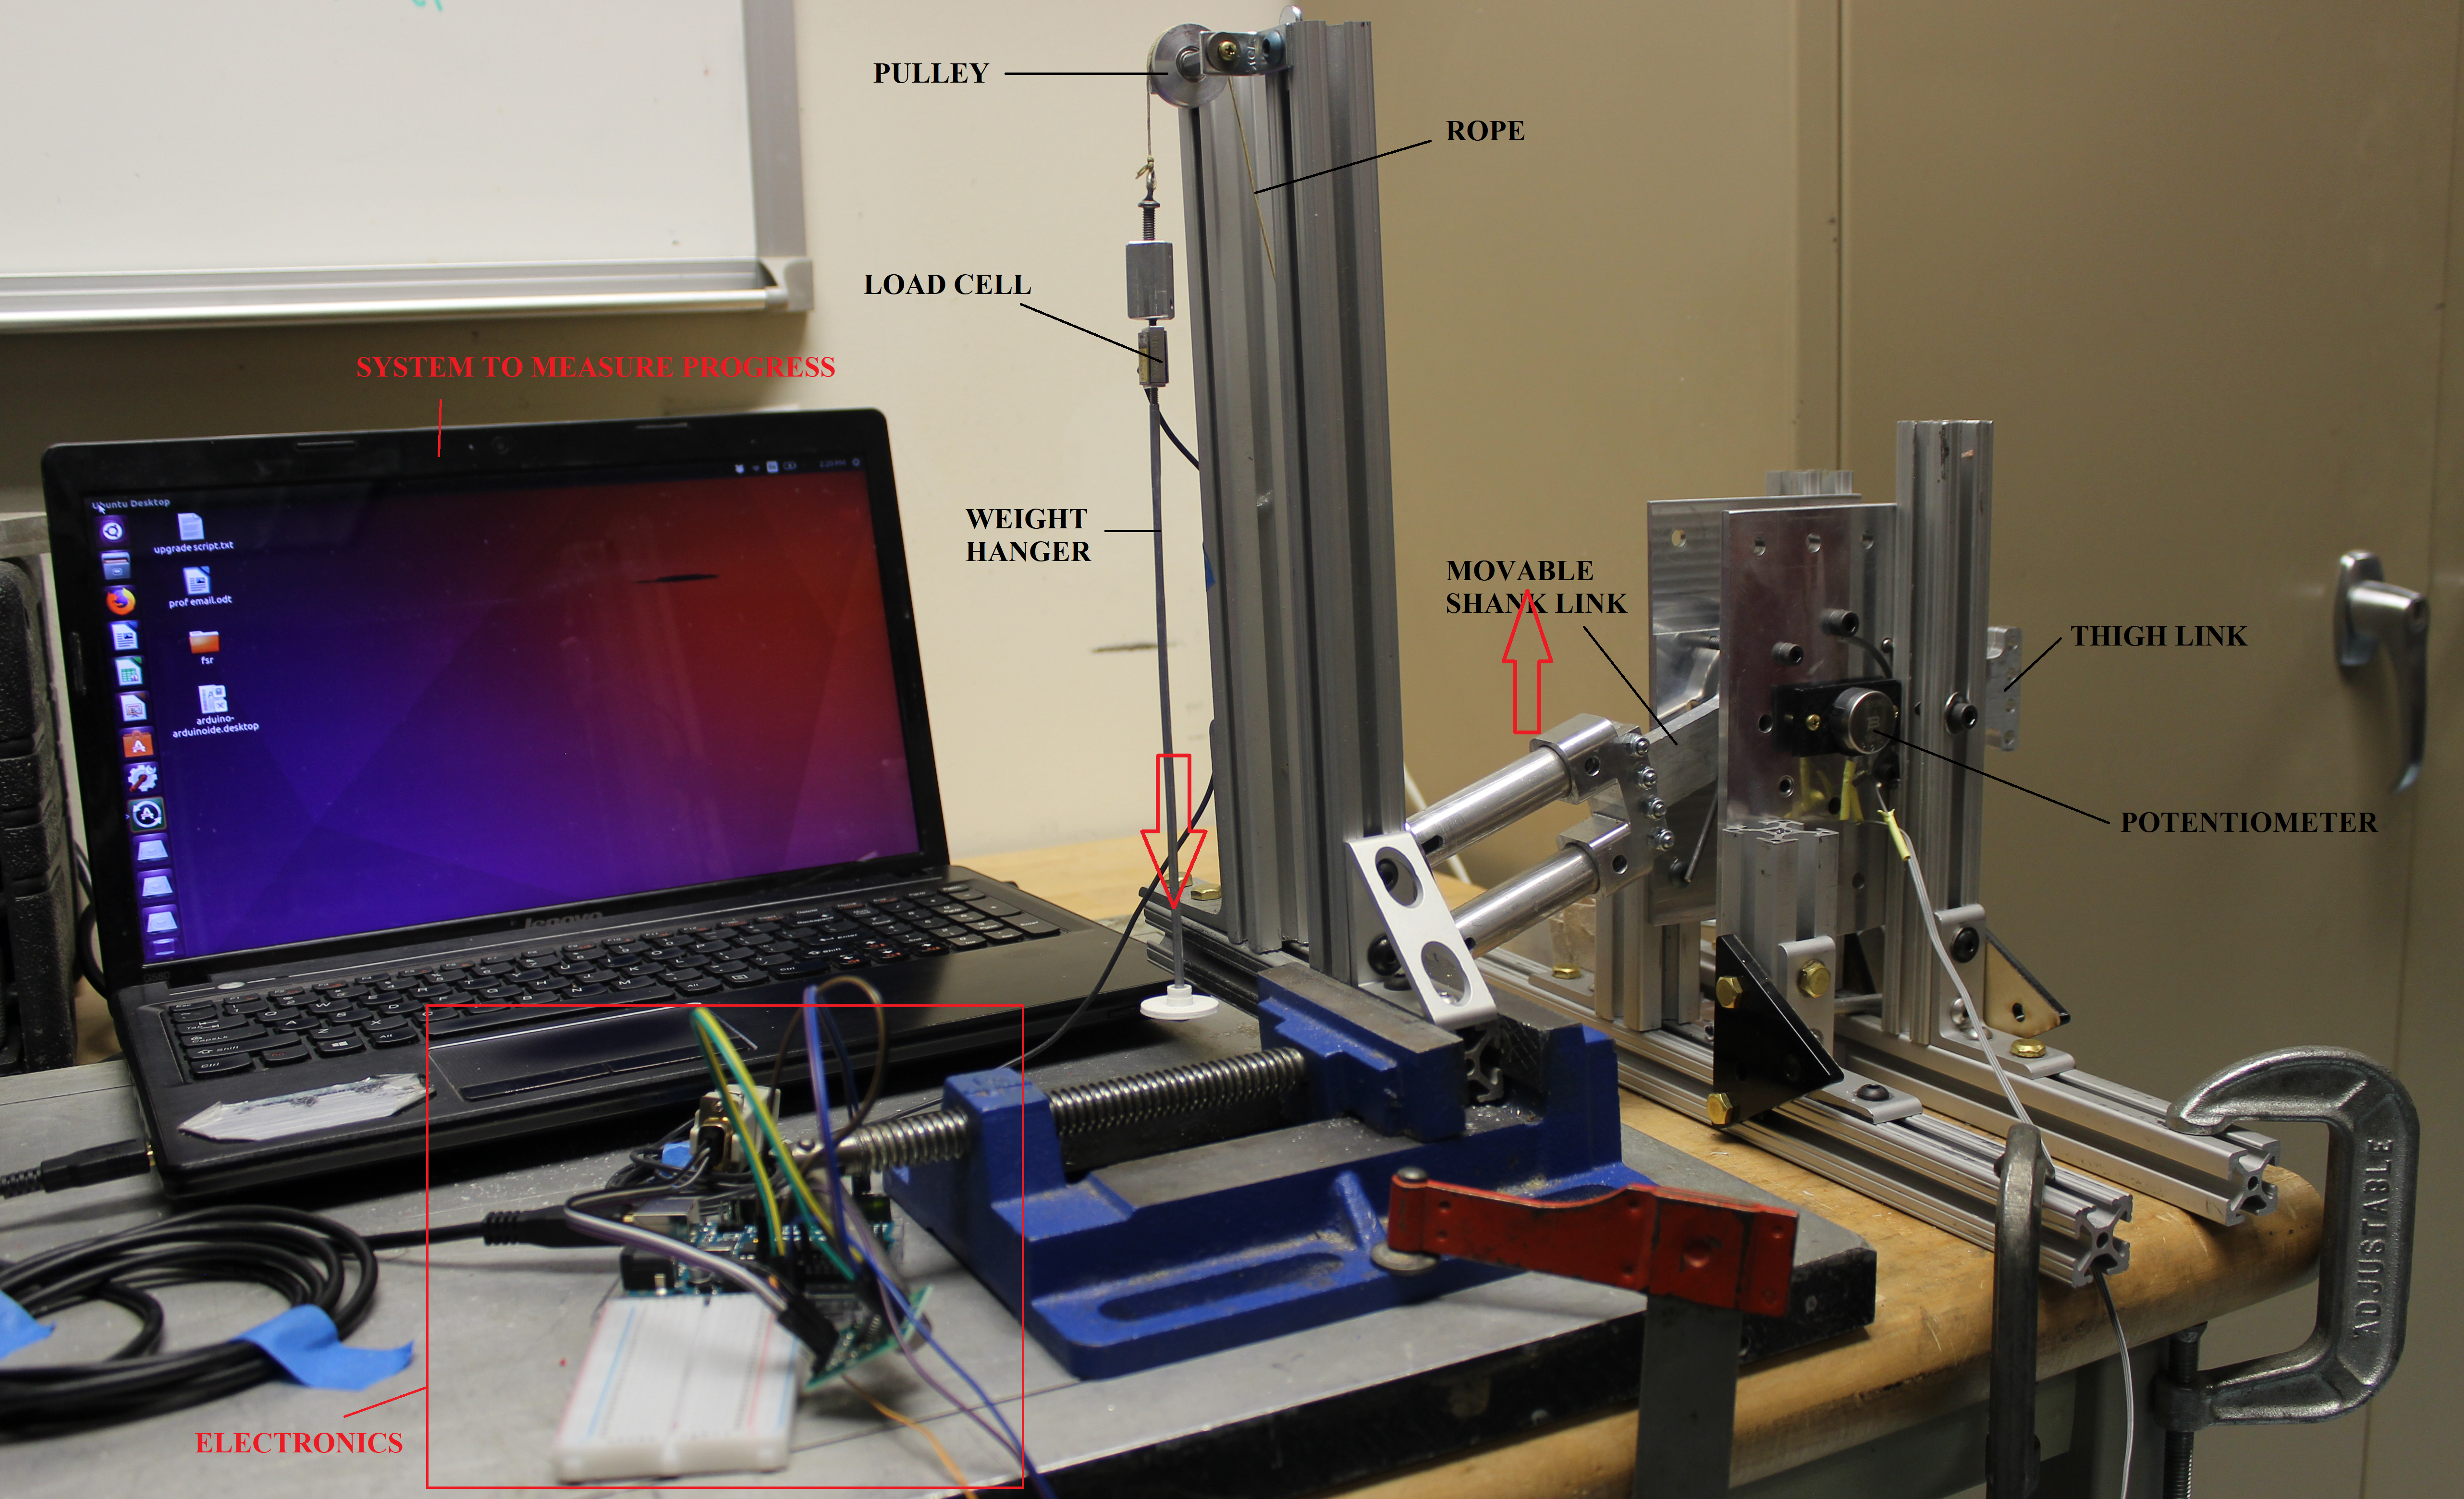
\includegraphics[scale=0.15]{images/mech_design/extension_set_up.png}
    \caption[Extension Test Bed]{Extension Test Bed}
    \label{fig:Extent_test_bed}
\end{figure}

This procedure was carried out for different interference values. The load values were substituted into \autoref{eq:ovTorque} to find the new interference values at which the slipped occurred.
\begin{equation}
    \large
    T_U & = p_0br^2(1 - e^{-N2\pi\mu})
\label{eq:ovTorque}
\end{equation}

The inner diameter of the spring is controlled by applying a force to the spring leg. Which also controls the interference between the arbor and spring. \autoref{fig:extension_test} shows the results of  
five different interference measurements. The black dots are the points of deflections for different spring openings. The $0push$ happens when the free spring leg is at its initial $0$ position. $1push$ happens when the spring leg is moved horizontally by a distance of $.313 in$ until $4push$.   

\begin{figure}[h!]
    \centering
    \includegraphics[scale=0.5]{images/mech_design/weighvspot.png}
    \caption[Knee Slipping Load Values]{Slipping Load values during Extension Test}
    \label{fig:extension_test}
\end{figure} 


\autoref{fig:Flexion_test_bed} shows the flexion test-bed used to estimate the static and dynamic holding torque behavior of the knee joint. The load applied direction, and the knee flexion direction was along the direction of gravity. The load on the knee was applied at a distance of $0.46m$ from the knee center. The load was applied over several days to measure the durability of the system. This test-bed was utilized to find RoM and the brake release force.



\begin{figure}[h]
    \centering
    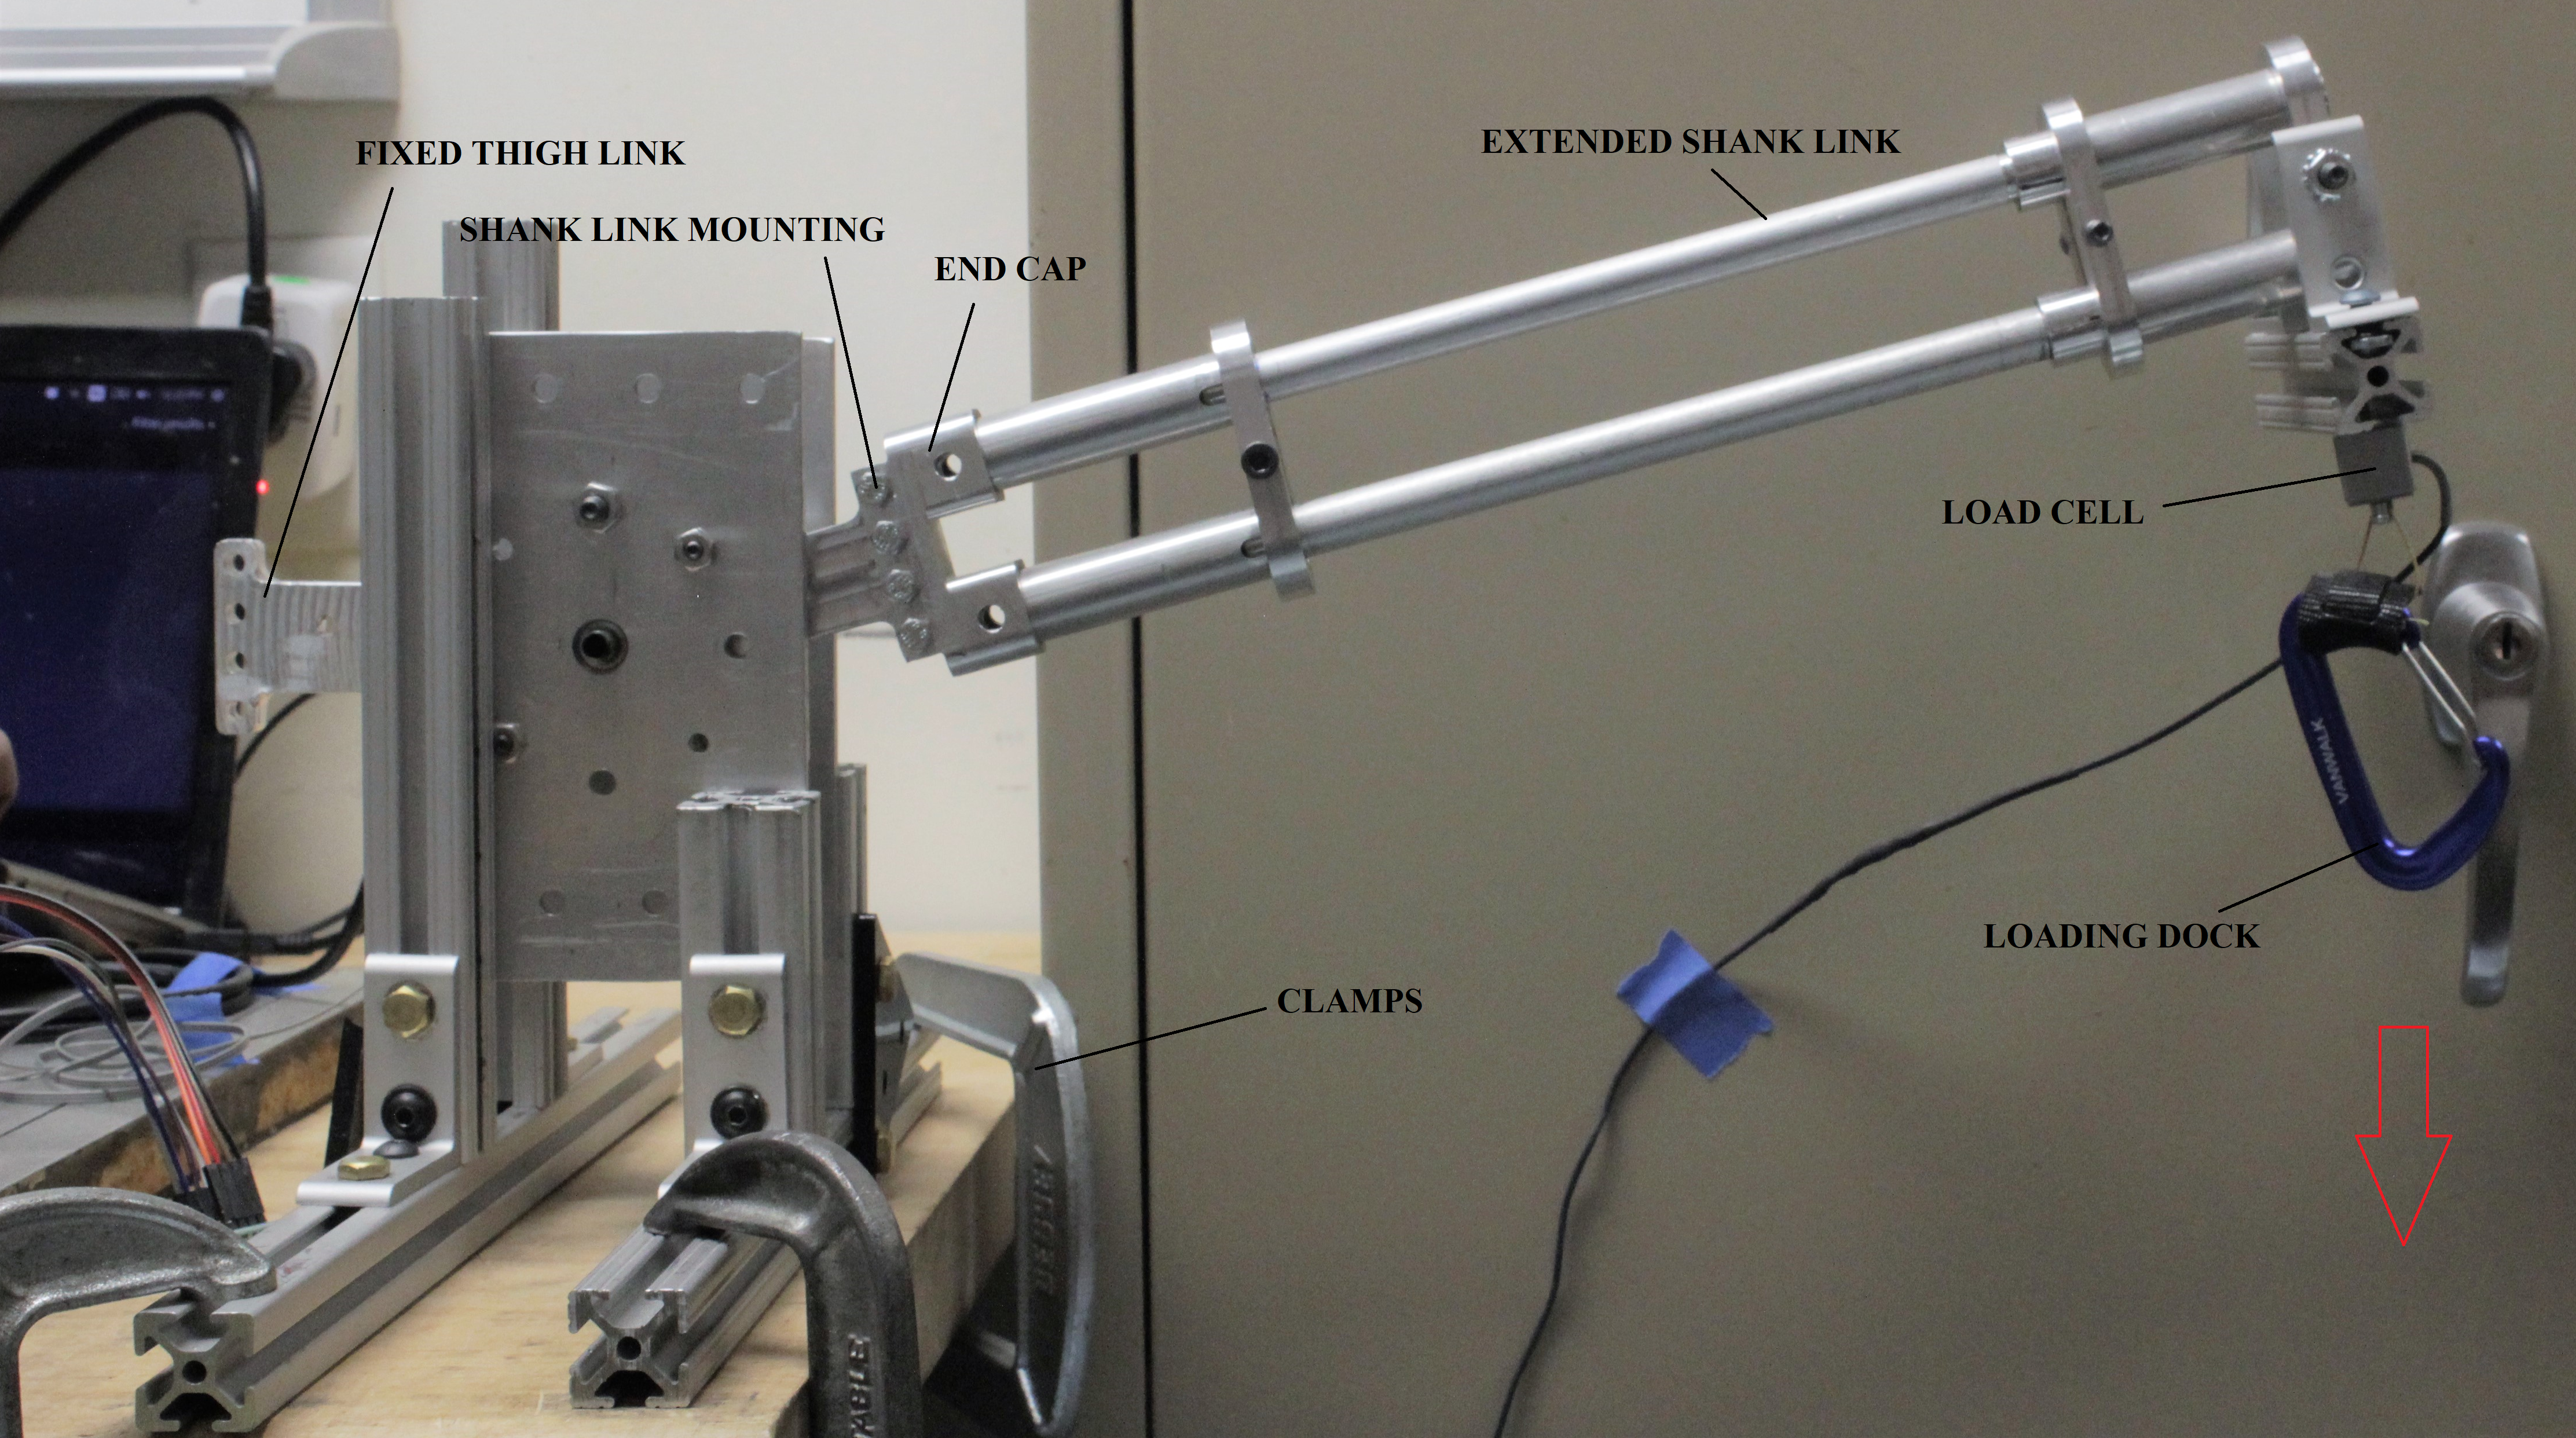
\includegraphics[scale=0.15]{images/mech_design/flexion_set_up.png}
    \caption[Flexion Test Bed]{Flexion Test Bed}
    \label{fig:Flexion_test_bed}
\end{figure}

The knee was loaded until the knee began to slip. The knee was found to have a maximum holding torque of $63Nm$, after which the knee started to slip. The knee was constructed to hold for an extended period of time, after which the knee lost 4$^{\circ}$ was observed, which was due to excessive stressing on the spring during maximum holding torque. The stress on the spring moved past its elastic region and entered the plastic region, due to which it was not able to coil back to its original position. \autoref{fig:loss_in_rom} shows the result of loss in the range of motion tests.
\begin{figure}[h!]
    \centering
    \includegraphics[scale=0.5]{ images/mech_design/loss_in_rom.png}
    \caption{Loss in Range of Motion}
    \label{fig:loss_in_rom}

\end{figure}

\autoref{fig:durabilitytest} shows the results of the durability test. During the test, the brake was engaged at three different loading conditions $48Nm$, $50Nm$, and $63Nm$. The brake was engaged to hold this position for four consecutive days, where the load between the days were increased; $48Nm$ on the first day, $50Nm$ for the second and third (since being the target requirement), and on the fourth day, we pushed the brake to the peak value of $63Nm$. The noise of the sensors was removed using a moving average filter.  The observed angular difference of the brake from the start of the test to the end was $0.75^{\circ}$.

\begin{figure}[h!]
    \centering
    \includegraphics[scale=0.50]{images/mech_design/Durability_test.png}
    \caption{Durability Test}
    \label{fig:durabilitytest}
\end{figure}


The testing results demonstrated that it is possible to build an analytical-based design approach for an actuator using biomechanical and predefined specifications.


The wrap spring clutch knee used an analytical-based design approach for the actuator selection. The knee developed for the LARRE is inexpensive and weighs less than  $1kg$. The system can be easily serviced or repaired. The detailed analytical model was used to identify the relationship between the parameters manipulated to improve the system's overall performance. The wrap spring clutch/brake mechanism underwent a wide range of testing to measure all the necessary knee joint characteristics. 

% \begin{figure}
% \centering
%      \begin{subfigure}{.45\textwidth}
%         \centering
%           \includegraphics[ scale=0.10]{images/mech_design/thigh_assembly2.png}
%     \caption[Thigh Sub-Assembly]{Thigh Sub-assembly: all components are labeled. The solenoid controls the activation of the brake.}
%     \label{fig:thigh_sub}
%     \end{subfigure} 
%     %
%      \begin{subfigure}{.45\textwidth}
%         \centering
%         \includegraphics[ scale=0.10]{images/mech_design/shank_assembly2.png}
%         \caption[Shank Sub-Assembly]{Shank Sub-assembly: The arbor interfaces with the spring. When the spring closes, it grabs the arbor and prevents rotation.}
%         \label{fig:shank_sub}
%     \end{subfigure}
%     \caption[Knee Sub-Assemblies]{The Knee sub-assemblies}
%     \label{fig:sub_knee}
% \end{figure}

\section{Prototype of personalized bio-mechanical knee}

The work done in this section was in collaboration with Alex Tacescu. I led and managed the focus of the project and came up with the idea. I was also involved with running the mocap experiments and the mechanical design. Another knee design was examined that focused on matching the knee motion profile to a human knee. Exoskeletons discussed in \autoref{sec:ExoBack} mostly use pin-type joints in their knee joints; this is in contrast to how the actual kinematics work in a human knew, which has a variable center of rotation \cite{morrison1970mechanics} \cite{koo2008knee}.

Several recent designs have focused more on accounting for knee motion. Choi \textit{et. al} used multiple rolling cams to adapt to the changing center of rotation \cite{choi2017development}. This design fits a person's knee motion; it did not use modeling of the knee's tibiofemoral motion to design the cams. Additionally, the design is complicated and not easily reproducible. In another design Choi \textit{et. al} used multiple rollers and pulleys powered by electric linear actuators. However, rotary electric motors with rotary gearboxes can often achieve higher performance than electric linear actuators powered by rotary DC motors. Another knee design was presented in \cite{wang2018comfort}; this design prioritized the comfort of the user and the alignment of the knee joint. This design also uses pulleys and cables to model the knee motion. \cite{AdaptiveKneeJoint} presents a cam knee design that uses a model of the knee motion. This design is a significant improvement over previous designs that merely compensate for the motion. However, as the other designs discussed, they use linear actuators.  These designs do well at either mimicking or compensating for the knee motion; however, they are mechanically cumbersome to manufacture; they did not show mimicking of the center of rotation's theoretical movement and/or use a linear actuator to replicate rotary motion. In addition, the design does not allow for the knee to be customized and therefore cannot meet the specific motion of the patient. Thus, we propose a knee design that is readily configured to match a particular patient's knee joint motion, is designed for easy manufacturing, and allows the use of readily available rotary actuators and brake mechanisms.

The variable center of rotation was found using previous work by Iwaki \textit{et. al} that used Magnetic Resonance Imaging (MRI) scans to determine and predict the knee's trajectory \cite{MRIKneeShape_Loaded, MRIKneeShape_Unloaded}. These studies used cadavers and actual patients to measure the motion of the knee in both loaded and unloaded scenarios. This MRI data was used in \cite{KinDynKneeJoint} to build a mathematical model of knee motion that considers both the flexion and extension degrees of freedom. They used ellipse to model the contact between the femur and tibia bones. Their work leads to the formulation of \autoref{eq:KneeExtensionFlexionNumeric}. This equation relates the rotation of the knee to the translation of the tibia. This motion and its derivative are shown in \autoref{fig:FlexExtRelationship}. This study was limited since it was based on the anthropomorphic parameters of a single person. These coefficients will vary slightly from person to person and can be found using MRIs or motion capture. 


\begin{equation}
    r(\theta) mm = 1.078\theta^4 - 11.184\theta^3 + 26.524\theta^2 - 0.825\theta + 263.59
    \label{eq:KneeExtensionFlexionNumeric}
\end{equation}

\begin{figure}[ht!]
    \centering
    \includegraphics[scale=0.9]{images/mech_design/FlexionCurve.png}
    \caption{Knee Flexion Curve}{Graphical representation of \autoref{eq:KneeExtensionFlexionNumeric} demonstrating the relationship between flexion and extension in a knee as measured by \cite{KinDynKneeJoint}. \(r(m)\) is the extension distance between the center of the knee and the center of mass of the lower leg. $0^\circ$ represents a perfectly extended knee joint.}
    \label{fig:FlexExtRelationship}
\end{figure} 

A cam-type mechanism with a brushless DC motor was designed to follow the desired path. The guide was generated using \autoref{eq:KneeExtensionFlexionNumeric}. This guide enforces variable center of rotation and motion of the tibia. \autoref{fig:ExplodedViewLabeled} shows an exploded view of the knee mechanism. 



\begin{figure}
    \begin{subfigure}{\textwidth}
        \centering
        \captionsetup{justification=centering}
        \includegraphics[scale=0.2]{images/mech_design/ExoKneeExplodedView.png}
        \caption{Bio Knee joint design exploded view}{Knee joint design exploded view}
        \label{fig:ExplodedViewLabeled}
    \end{subfigure}
    \begin{subfigure}{\textwidth}
        \centering
         \includegraphics[scale=0.2]{images/mech_design/KneeJointAssyCrossSection.png}
          \captionsetup{justification=centering}
        \caption{Cross section of Bio knee}{A cross section of the knee joint with the potentiometer embedded in the design. The wires are routed along the wire channel to avoid interference with the inner arm and plastic slides}
        \label{fig:CrossSectionPot}
    \end{subfigure}    
    \caption{Exploded View of bio-knee mechanism}
    \label{fig:bioknee}
\end{figure}

The motor and gearbox need to provide sufficient torque and power to drive the knee of a $100kg$ patient through gait motion. This mass is larger than the average mass of the North American paraplegic, which is $68.8kg$, so assuming a larger mass allows for the motor to have a safety factor. Additionally, it is assumed that the dynamic loads are assumed to be negligible during the slow-motion collision with the ground. It equates to approximately $65W$ of power and $25Nm$ of torque at \(15^\circ/sec\). The knee is powered by a $90W$ brushless Maxon motor used with a nominal torque of $0.56Nm$ at roughly $2500rpm$.  The motor is combined with a Harmonic gearbox with a $100:1$ reduction. \autoref{table:MotorGearboxSpecs} shows the gearbox and motor specifications and the joint's mechanical properties. The calculations assumed an efficiency of \(90\%\) as per the manufacturer documentation. The designed knee joint can mechanically output $81W$ and $50.4Nm$ at $15^\circ/sec$.  

\begin{table}
    \centering
    \begin{tabular}{||c|c|c||}
        \hline
        Input (Motor) Power & \(P_{input}\) & \(90 Watts\) \\
        \hline
        Input (Motor) Torque @ Nominal & \(\tau_{input}\) & \(0.560 Nm\) \\
        \hline
        Input (Motor) Speed @ Nominal & \(\omega_{input}\) & \(2510 rpm\) \\
        \hline
        Input (Motor) Stall Torque & \(\tau_{in\_stall}\) & \(7.480 Nm\) \\
        \hline \hline
        Gearbox Ratio & \(\frac{n_1}{n_2}\) & \(100:1\) \\
        \hline \hline
        Output Power & \(P_{output}\) & \(81 Watts\) \\
        \hline
        Output Torque @ Nominal & \(\tau_{input}\) & \(50.4 Nm\) \\
        \hline
        Output Speed @ Nominal & \(\omega_{input}\) & \(15^\circ/sec\) \\
        \hline
        Output Stall Torque & \(\tau_{out\_stall}\) & \(673.2 Nm\) \\
        \hline
    \end{tabular}
    \caption{Bio Knee parameters}{Motor/gearbox specifications and output power specifications of the proposed joint.}
    \label{table:MotorGearboxSpecs}
\end{table}

The design was validated using a motion capture system and SolidWorks motion analysis \footnote{https://www.solidworks.com/category/simulation-solutions}. The markers on the knee were aligned on the shank and thigh segments of the knee and rotated through the desired motion as shown in \autoref{fig:KneeJointTestSetup}; this allowed us to compare the theoretical trajectory to the actual trajectory, and for the measurement and comparison of manufacturing tolerance. \autoref{fig:KneeJointTestResults} shows the results of the study. There are some slight deviations of the actual motion compared to the desired motion; this deviation is caused by hysteresis in the system. However, these movements are very slight on a scale of less than $1mm$, which is assumed to be negligible.   



\begin{figure}[ht!]
    \centering
    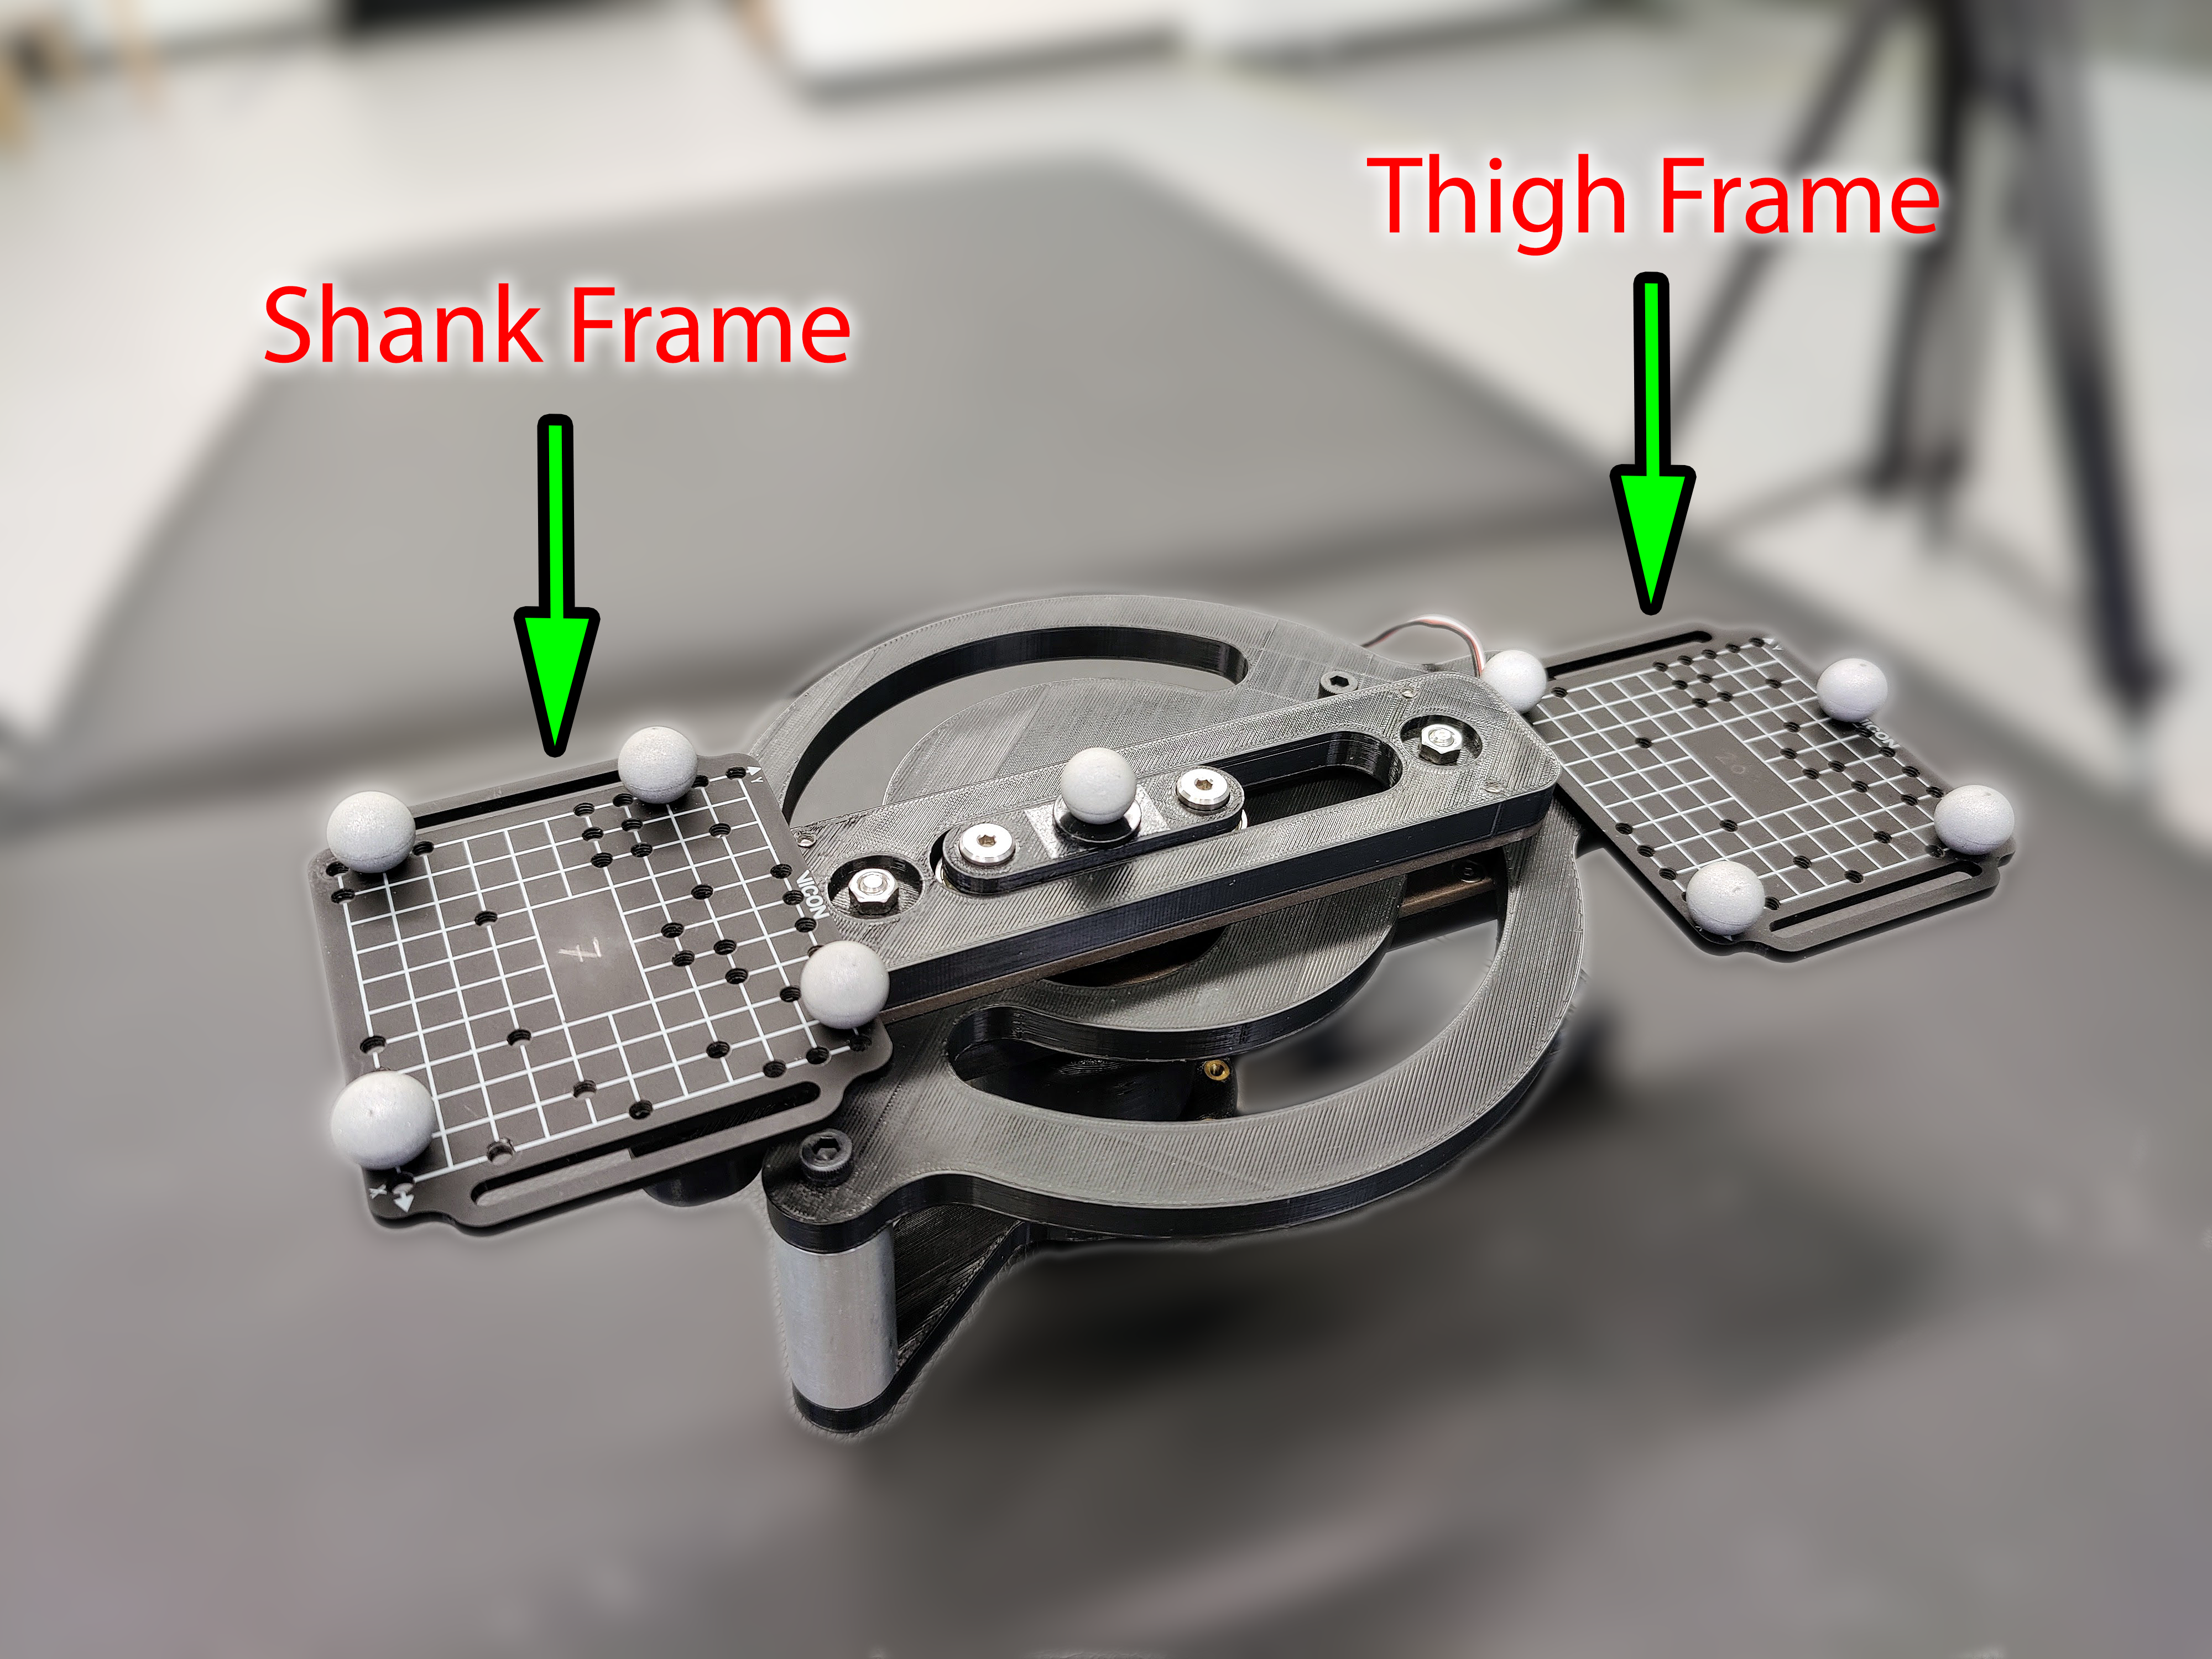
\includegraphics[scale=0.07]{images/mech_design/KneeTrajTest_edit.png}
    \caption{Knee with mocap markers}{Knee joint setup with motion capture dots}
    \label{fig:KneeJointTestSetup}
\end{figure}

\begin{figure}[ht!]
    \centering
    \includegraphics[scale=0.75]{images/mech_design/FlexionExtensionKneeJoint.png}
    \caption{Comparison of variable center of rotation}{Graph showing knee joint flexion vs linear extension of the radius of curvature for the goal trajectory (see \autoref{eq:KneeExtensionFlexionNumeric}) and the experimental results from the Motion Capture Study}
    \label{fig:KneeJointTestResults}
\end{figure}

This knee design is easily manufactured; the common parts are made from off-the-shelf parts. The only customizable component is the guide plate, 3D printed on a standard 3D printer. The path can be fitted to the individual's anthropomorphic parameters, 3D printed without understanding advanced manufacturing methods of techniques. 

\section{Ankle Foot Orthosis}
\label{sec:ankle}
The work done in this section was in collaboration with Nathaniel Michaels. I was the lead designer and gave feedback for the mechanical and electrical design. I also designed and helped run the experiments for the validation of the systems. 

The ankle-foot orthosis (AFO) of LARRE comprises two components, a passive ankle joint to keep the foot straight and a sensor to sense the ground force reactions. The design process of the AFO is discussed in more detail here \cite{Michaels2020}.  A rendering of the AFO mechanism is shown in \autoref{fig:AFO Mechanism Full} and \autoref{fig:Outer Ankle Box fig}. The AFO is designed to fit over the shoe to allow the operator to easily donn and doff the exoskeleton, uses a passive spring to balance the foot's mass and prevent foot drop while still allowing flexion, and the sensing sole detects the phases of the gait cycle. 

\begin{figure}[h!]
    \centering
    \begin{subfigure}[b]{0.45\textwidth}
        \centering
        \captionsetup{justification=centering}
        \centerline{
        \includegraphics[scale=0.2]{images/mech_design/AFO_Exploded_AND_Force_Sole_WITH_Labels2.png}}
        \caption{AFO Mechanism. There are three parts to the system; the outer ankle box, the sensing sole, and the the metal foot plate}
        \label{fig:AFO Mechanism Full}
    \end{subfigure}
    %
    \begin{subfigure}[b]{.45\textwidth}
        \centering
        \captionsetup{justification=centering}
        \centerline{
        \includegraphics[scale=0.15]{images/mech_design/Outer_Ankle_Box_Exploded_WITH_Labels2.png}}
        \caption{Outer Ankle Box Exploded View. This system transfers the body load from the legs to the floor. The spring }
        \label{fig:Outer Ankle Box fig}
    \end{subfigure}%
    \caption{AFO Sub-Assemblies}
    \label{fig:AFO Sub-Assemblies}
\end{figure}


The sensing sole has Ohmite FSR03C3 Force Sensing Resistors (FSRs) \footnote{https://www.ohmite.com/catalog/fsr-series/FSR03CE} embedded into the toe and heel areas of the sole. FSRs are flat flexible resistors that change their electrical resistance based on the applied force \cite{yaniger1991force} and convert the force to an electrical signal by measuring the sensor's variation of conductivity. The small flexible forum factor force-sensing makes them ideal sensors for wearable devices \cite{giovanelli2016force}.    

FSRs embedded into the sole of an AFO can measure the gait phases. Patar \textit{et. al} two embedded FSRs into their AFO to measure the transition pressure points in the foot during the gait cycle\cite{ab2014system}. In their model, a single FSR was placed on the foot's heel and ball, respectively.  

\autoref{fig:Foot-Force Mapping} shows the sensors' locations relative to the pressure points. The FSRs are encased in a Urethane risen. The risen distributes the ground forces onto the sole and protects the sensors from being damaged. The resin has properties similar to shoes' soles, with a shore hardness of 20 and a non-stick surface \footnote{Vytaflex20Website}. Both Vytaflex-20 \footnote{https://www.smooth-on.com/products/vytaflex-20/} and Vytaflex-30 \footnote{https://www.smooth-on.com/products/vytaflex-30/} were tested as possible options. Once the system was cured, the Vytaflex-30 material had a sticky surface texture. It was not suitable since contact with the ground and dirt and debris would stick to the surface. The Vytaflex-20 material was cured with a surface and was much less sticky, making it better than the Vytaflex-30 material for encasing the sole sensors. 

The Vicon motion capture system and the AMTI force plates were used to measure the center of pressure of the AFO.  The measurement was used to detect the individual reading of the FSR and to validate the AFO's CoP. Each of the FSR's was treated as an on-off switch. If the pressure detected was above a threshold, it was treated as "on," below the threshold as "off."  Several different versions of the AFO were tested; the final version of the sensors readings and filtering is shown in \autoref{fig:FSRBinarized}. As shown, the filtering removes the noise from the sensor reading. \autoref{tab:statetable} shows a state table to detect the different states of the AFO. 

\begin{figure}[h!]
    \centering
    \includegraphics[scale=0.45]{images/mech_design/SoleSensorV3T2_Raw_v_Binarized.png}
    \caption[Measurement of raw FSR]{Measurement of raw FSR activation and filtering \cite{Michaels2020}}
    \label{fig:FSRBinarized}
\end{figure}


\begin{table}[h!]
    \centering
    \begin{tabular}{|c|c|c|c|}
    \hline
    FSR1 - Inner Ball & FSR2 - Outer Ball & FSR3 - Heel & Position-State \\[0.5ex]
    \hline\hline
    0 & 0 & 0 & Foot not on ground \\
    \hline
    0 & 0 & 1 & Heel-Down \\
    \hline
    0 & 1 & 0 & Transition or Error \\
    \hline
    0 & 1 & 1 & Leaning Outward \\
    \hline
    1 & 0 & 0 & Transition or Error \\
    \hline
    1 & 0 & 1 & Leaning Inward \\
    \hline
    1 & 1 & 0 & Toe-Down \\
    \hline
    1 & 1 & 1 & Flat-Foot \\
    \hline
    \end{tabular}
    \caption[AFO State Table]{AFO Position State-Table with FSRs as bits \cite{Michaels2020}}
    \label{tab:statetable}
\end{table}



\begin{figure}[h!]
    \centering
    \includegraphics[scale=0.25, angle =-90 , frame]{images/mech_design/sole.png}
    \caption[Pressure Map of Foot]{Overlay of Pressure Map with current Foot Sensor design}
    \label{fig:Foot-Force Mapping}
\end{figure}

Finite element analysis (FEA) was used to validate that the AFO could withstand the applied forces \cite{akin2010finite}. The FEA analysis was conducted using SolidWorks \footnote{https://www.solidworks.com/} FEA tools; this allowed for each of the individual components to be tested and validated before being manufactured. The testing showed that components under the assumed loads, the Von Mises \cite{shigley} stress, did not exceed the materials' yield strength and would not break.

\begin{equation}
\large
    \{x,y\}_{cop} = \sum_{i}^{N} \{x,y\}_i F_i
    \label{eq:FSRCoP}
\end{equation}

The Center of Pressure (CoP) of the AFO is measured by using \autoref{eq:FSRCoP}, where $\{x,y\}$ is the location of the FSR and $F$ is the force of the FSR. The location of FSRs is shown in \autoref{fig:AFOmocap}. The CoP was validated using the mocap and force plates. The force was measured using the force plate, which provides the force along each axis, and the mocap markers located the force vectors in space. The mocap+forceplates were used to dead reckon the FSR sensors. 




 \begin{figure}[h]
    \ContinuedFloat
           \captionsetup{justification=centering}
           \centerline{ \includegraphics[scale=0.22]{images/mech_design/Mocap_Layout_2.png}}
            \caption[AFO Mocap Markers]{Location of mocap markers and FSRs on the AFO \cite{Michaels2020}}
            \label{fig:AFOmocap}
    \end{figure}


The results of the CoP measurement are summarized in \autoref{fig:3DFSRCoP} and \autoref{fig:FSRCoPAFO} . The shape created by the AFO point shows major distortions across the $x$ axis compared to the force plate. The $z$ axis can be ignored since it is perpendicular to the page and has no significant meaning. The major axis of interest is the $y$ axis that goes along the foot's cardinal longitudinal axis. These FSRs can track the CoP measured by the force plates. 


\begin{figure}[h!]
    \centering
    \begin{subfigure}{0.5\linewidth}
        \captionsetup{justification=centering}
        \centerline{ \includegraphics[scale=0.35]{images/mech_design/SoleSensorV3_CoPComparison_2D_XYplane.png}}
        \caption[CoP comparison]{The CoP comparison results between the calculated AFO CoP point and the Force-Plate CoP point within the world frame, across both trials.}
        \label{fig:3DFSRCoP}
    \end{subfigure}%
    \vspace{1cm}
    \begin{subfigure}{.5\linewidth}
        \captionsetup{justification=centering}
        \centerline{\includegraphics[scale=0.35]{images/mech_design/SoleSensorV3_CoPComparison_BothTrials.png}}
        \caption[CoP Point Trail ]{CoP Point trail created by both the Force-Plates and AFO across both trials. }
        \label{fig:FSRCoPAFO}
    \end{subfigure}%
    \caption[Center of Pressure of the AFO]{Center of pressure of the AFO measured using the FSRs compared to the forceplate measurement \cite{Michaels2020}}
    \label{fig:CoPAFO}
\end{figure}


This device combined passive-dorsiflexion control methods and sensory feedback systems into a single AFO device for LARRE. This device acts as a fully-functional DAFO device capable of controlling foot-drop using a passive torsional-spring system. The devices provide real-time feedback for balance control and force distribution.  Using three FSRs instead of two makes it possible to determine the CoP point within the support polygon they form.  This information can be used by the main controller onboard the LARRE to help the system maintain its balance.


\section{Final Design}

LARRE's leg segments are constructed from 6061 aluminum alloy concentric sliding pipes with clamps allowing the joints' to be adjusted for each person. This material is lightweight and easy to manufacture. The axles of the joints were constructed of steel to handle the expected stress. Safety is a significant concern; careful attention was given to the manufacturing process to minimize the sharp edges since it is attached to a human-machine interface system. Safety is essential for people with SCI who have minimal sensory abilities and would not feel an injury.  LARRE is attached to a person through the upper body and waist straps. Custom-made 3D printed strap carriages are placed on the thigh and shank segment and connect the person to the exoskeleton's legs. \autoref{fig:LARRE} shows the final model of LARRE.     


\begin{figure}
    \centering
    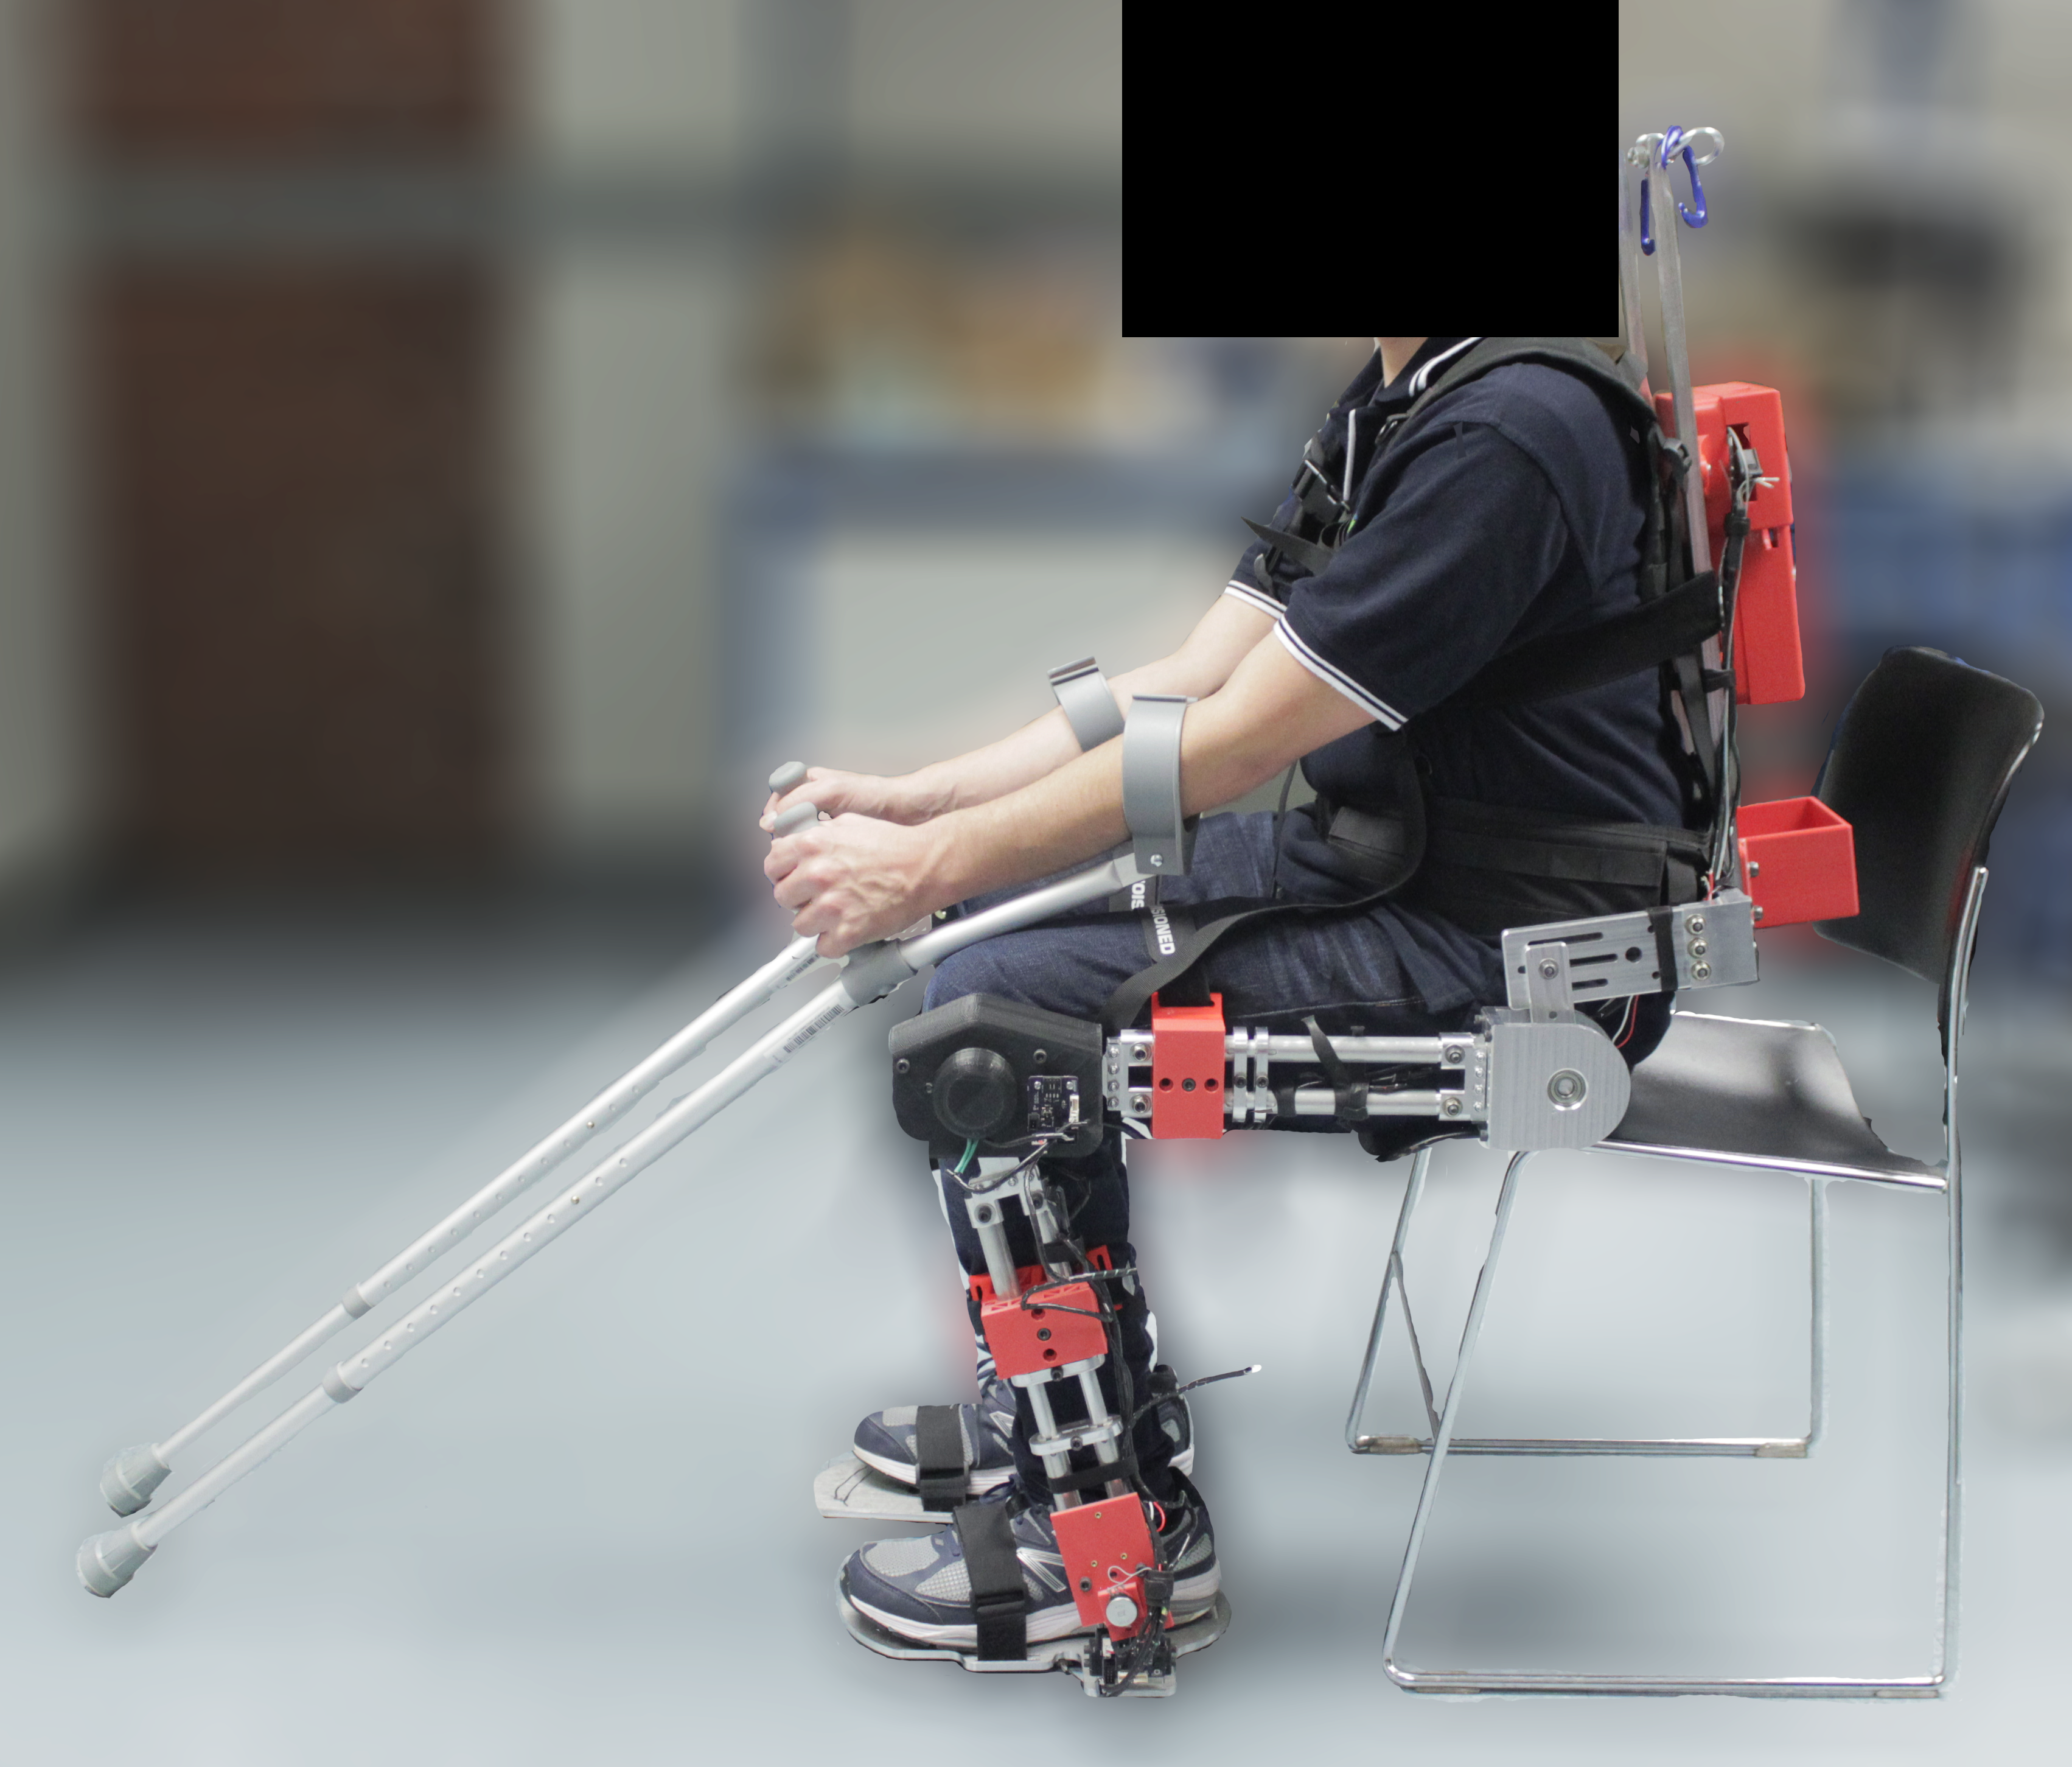
\includegraphics[scale=0.08]{images/mech_design/exo_side2.png}
    \caption{The LARRE exoskeleton being worn}
    \label{fig:LARRE}
\end{figure}


The dynamic properties of LARRE are essential for building the controller. The dynamics of LARRE were calculated using SolidWorks. The properties account for the material properties of the components as well as the geometry. \autoref{tab:LARREMASS} summarizes the dynamic properties of LARRE. The exoskeleton has defined joint limits to allow for biological motion, summarized in \autoref{tab:jointlimits}.

\begin{table}[h!]
    \centering
    \begin{tabular}{|c c c c c|}  
         \hline 
          \multicolumn{5}{|c|}{Exoskeleton Segment Parameters} \\
         \hline
         Link & Mass (kg) & $CoM_x$ & $CoM_y$ & $CoM_z$ \\
         \hline \hline
         Hip & 2.3677 & 0.000011338 & 0.093937 &  -0.12619 \\
         Thigh & 2.1138 & 0.0034745   & 0.097979 &  0.1712 \\
         Shank & 1.2804  &   0.002761 & 0.097563   & 0.15581\\
         Foot & 0.85523 & 0.14092 & 0.2267 &  -0.31138  \\
         \hline
    \end{tabular}    
    \caption[Dynamic Properties of the LARRE]{Mass Properties of the LARRE}
    \label{tab:LARREMASS}
\end{table}


\begin{table}[h!]
\begin{centering}
    \begin{tabular}{ |p{1cm} p{2cm} p{2cm} |  }
        \hline 
        \multicolumn{3}{|c|}{LARRE Joints Limits} \\
        \hline 
        Joint & Flexion & Extension \\
        \hline \hline
        Hip   & $-60^{\circ}$   & $30^{\circ}$  \\
        Knee &   $-110^{\circ}$  & $0$   \\
        Ankle & $-20^{\circ}$ & $20^{\circ}$  \\
        \hline
    \end{tabular}
    \caption[LARRE Joint Limits]{Joint limits}    \centering
    \label{tab:jointlimits}
\end{centering}
\end{table}


A single patient study was conducted to measure the kinematics and dynamics of a gait while wearing LARRE. This study was not designed to measure the ability of the exoskeleton to induce movement but merely to observe the motion of the exoskeleton. The Vicon setup described in \autoref{sec:setup} was used with the custom marker layout shown in \autoref{fig:larremarker}. Additional markers were added to the plug-in gait model. \autoref{tab:exomarkerlayout} details the rigid bodies used and their location (see \autoref{fig:markers} for definition of the marker layout). The additional markers were added to ensure that there was no marker occlusion during the trial. 


\begin{table}[h!]
    \begin{centering}
            \begin{tabular}{||c  c ||} 
         \hline
            Plate Name & Plate \#  \\ [0.5ex] 
            \hline\hline
            LTHIGH	& 11 \\
            LSHANK &	19\\
            LFOOT &	9 \\
            LTHIGH FRONT &	7\\
            LTHIGH BACK &	15\\
            LSHANK FRONT &	4\\
            LSHANK BACK &	14\\
            RTHIGH SIDE &	5\\
            RSHANK SIDE &	17\\
            RFOOT &	10\\
            RTHIGH FRONT &	20\\
            RTHIGH BACK &	16\\
            RSHANK FRONT &	1\\
            RSHANK BACK &	3\\
            BACK &	2\\ [1ex] 
         \hline
        \end{tabular}
        \caption[Exoskeleton Rigid Body Numbers]{Rigid Body Numbers}
        \label{tab:exomarkerlayout}
    \end{centering}
\end{table}

The joint kinematics are shown in \autoref{fig:exojointkin}. Only a single demonstration is shown; however, multiple demonstrations were recorded. Similarly, data were recorded for both legs, but just the right leg is shown. The heel strikes and toe-offs are pointed out in the graphs. These points are calculated using the Vicon plug-in gait tools. All of the data presented were extracted and analyzed using the tools discussed in \autoref{chap:software}. In this study, three steps were taken across the mocap floor. The first step was slightly off since it started with feet together; however, steps two and three aligned with the expected motion. The gait cycles are presented over the collected frames; the Vicon records at $100fps$, so the presented trial is approximately $14.04s$. LARRE was able to move through the desired joint range for a gait cycle. Similarly, with the moments shown in \autoref{fig:larregaitmoments}, the first step did not contain relevant data since the moments can only be calculated when the force plates embedded on the floor are stepped on. The moments are presented in $\frac{Nm}{Kg}$ which allows for the torque to be abstracted and calculated for the different masses. 








\begin{figure}[h!]
    \begin{subfigure}{0.5\textwidth}
        \centering
        \captionsetup{justification=centering}
        \centerline{
        \includegraphics[scale=0.1, frame]{images/mech_design/exo_markers_back.png}}
        \caption[LARRE marker set back/side]{LARRE marker set back/side}
        \label{fig:larremarkerside}
    \end{subfigure}
    \begin{subfigure}{0.5\textwidth}
        \centering
        \captionsetup{justification=centering}
        \centerline{
        \includegraphics[scale=0.1, frame]{images/mech_design/exo_markers_front.png}}
        \caption[LARRE marker set front]{LARRE marker set front}
        \label{fig:larremarkerfront}
    \end{subfigure}    
    \caption{Marker set for LARRE}
    \label{fig:larremarker}
\end{figure}



\begin{figure}
    \begin{subfigure}{\textwidth}
        \centering
        \captionsetup{justification=centering}
        \centerline{
        \includegraphics[width=\textwidth, frame]{images/mech_design/exo_joint_angles.png}}
        \caption[LARRE gait cycle angles]{Gait cycle angles of the LARRE}
        \label{fig:larregaitangles}
    \end{subfigure}
    \begin{subfigure}{\textwidth}
        \centering
        \captionsetup{justification=centering}
        \centerline{
        \includegraphics[width=\textwidth, frame]{images/mech_design/exo_joint_moments.png}}
        \caption[LARRE gait cycle moments]{Gait cycle moments of the LARRE}
        \label{fig:larregaitmoments}
    \end{subfigure}
    \caption{Gait cycles kinematics for LARRE}
    \label{fig:exojointkin}
\end{figure}




\autoref{fig:positioncomparison} compares the position of the LARRE to the that human. The positional difference has a maximum displacement between $10mm-20mm$. \autoref{fig:markerpositiondiagram} shows a diagram of the marker position on the thigh segment and LARRE with a simplified model that illustrates the calculation.  This difference was measured be using the front and back rigid body plates on the legs and on the side of the exoskeleton. The centroid of the front/back markers was taken as the location of that body segment. The mean position was removed to only show the average change in position over the course of the trial.  

\begin{figure}[h!]

    \begin{subfigure}{\textwidth}
        \centering
        \captionsetup{justification=centering}
        \centerline{
        \includegraphics[width=\textwidth, frame]{images/mech_design/position_comparison.png}}
        \caption[Comparison of Difference of Human and LARRE Position]{Comparison of the human position vs. LARRE position}
        \label{fig:positioncomparison}
    \end{subfigure}
        \begin{subfigure}{\textwidth}
        \centering
        \captionsetup{justification=centering}
        \centerline{
        \includegraphics[width=0.5\textwidth, frame]{images/mech_design/side_marker_positioning.png}}
        \caption[Diagram of Marker Segment Measurement]{Diagram of Marker Segment Measurement}
        \label{fig:markerpositiondiagram}
    \end{subfigure}
    \caption[Comparison of LARRE and human positions]{Comparison of the positional difference of LARRE and the human.}
    \label{fig:exohumanmarkercompare}
\end{figure}


The electrical control system for LARRE is currently under development. The control board was developed by Micheal Conrad. The control board consists of a  Xilinx Zynq 7000 \footnote{https://www.xilinx.com/products/silicon-devices/soc/zynq-7000.html}  field-programmable gate arrays (FPGAs) as the primary controller for the exoskeleton. This allows for high speed communication with the motors and sensors. The control board is shown in[insert control board figure].

Additionally, custom PCB with integrated inertial measurement unit (IMU) and potentiometer connectors are placed on each of the leg segments (thigh, shank, and foot). The PCM is shown in \autoref{fig:imu_circut} Cables run down from the main control board the leg and snap into each of the IMU boards. This allows for the collection of all the sensor information.  

\begin{figure}
    \centering
    \includegraphics[scale=0.18]{images/mech_design/IMU_circut_edit.png}
    \caption{IMU circuit diagram}
    \label{fig:imu_circut}
\end{figure}

% \begin{table}[h!]
% \begin{centering}
%     \begin{tabular}{ |p{1cm} p{2cm} p{2cm} p{2cm}|  }
%         \hline 
%         \multicolumn{4}{|c|}{LARRE Joints Limits} \\
%         \hline 
%         Joint & Flexion & Extension & Torque \\
%         \hline \hline
%         Hip   & $-60^{\circ}$   & $30^{\circ}$ &  60N \\
%         Knee &   $-110^{\circ}$  & $0$  & 50N \\
%         Ankle & $-20^{\circ}$ & $20^{\circ}$ &  - \\
%         \hline
%     \end{tabular}
%     \caption[LARRE Joint Limits]{Joint limits}    \centering
%     \label{tab:biomech}
% \end{centering}
% \end{table}



\section{Contributions}

The developed exoskeleton allows for a modular and comprehensive method to test and develop different joints mechanisms. The modular connection interfaces allowed for the development of several different mechanisms. The mechanical design and SolidWorks parts were released open source for the community to use. By providing the basic mechanical structure, researchers can put more effort into constructing new sensors and mechanical actuators instead of the entire system. The platform also allows for adjustment to the user. The legs can be extended to fit the person's legs, and the hip-width can be expanded to ensure a good fit. This feature is critical for testing the exoskeleton on different people.  

